%%%%%%%%%%%%%%%%%%%%%%%%%%%%%%%%%%%%%%%%%
% The Legrand Orange Book
% LaTeX Template
% Version 2.4 (26/09/2018)
%
% This template was downloaded from:
% http://www.LaTeXTemplates.com
%
% Original author:
% Mathias Legrand (legrand.mathias@gmail.com) with modifications by:
% Vel (vel@latextemplates.com)
%
% License:
% CC BY-NC-SA 3.0 (http://creativecommons.org/licenses/by-nc-sa/3.0/)
%
% Compiling this template:
% This template uses biber for its bibliography and makeindex for its index.
% When you first open the template, compile it from the command line with the 
% commands below to make sure your LaTeX distribution is configured correctly:
%
% 1) pdflatex main
% 2) makeindex main.idx -s StyleInd.ist
% 3) biber main
% 4) pdflatex main x 2
%
% After this, when you wish to update the bibliography/index use the appropriate
% command above and make sure to compile with pdflatex several times 
% afterwards to propagate your changes to the document.
%
% This template also uses a number of packages which may need to be
% updated to the newest versions for the template to compile. It is strongly
% recommended you update your LaTeX distribution if you have any
% compilation errors.
%
% Important note:
% Chapter heading images should have a 2:1 width:height ratio,
% e.g. 920px width and 460px height.
%
%%%%%%%%%%%%%%%%%%%%%%%%%%%%%%%%%%%%%%%%%

%----------------------------------------------------------------------------------------
%	PACKAGES AND OTHER DOCUMENT CONFIGURATIONS
%----------------------------------------------------------------------------------------

\documentclass[11pt,fleqn]{book} % Default font size and left-justified equations

%%%%%%%%%%%%%%%%%%%%%%%%%%%%%%%%%%%%%%%%%
% The Legrand Orange Book
% Structural Definitions File
% Version 2.1 (26/09/2018)
%
% Original author:
% Mathias Legrand (legrand.mathias@gmail.com) with modifications by:
% Vel (vel@latextemplates.com)
% 
% This file was downloaded from:
% http://www.LaTeXTemplates.com
%
% License:
% CC BY-NC-SA 3.0 (http://creativecommons.org/licenses/by-nc-sa/3.0/)
%
%%%%%%%%%%%%%%%%%%%%%%%%%%%%%%%%%%%%%%%%%

%----------------------------------------------------------------------------------------
%	VARIOUS REQUIRED PACKAGES AND CONFIGURATIONS
%----------------------------------------------------------------------------------------

\usepackage{graphicx} % Required for including pictures
%\graphicspath{{Pictures/}} % Specifies the directory where pictures are stored

\usepackage{lipsum} % Inserts dummy text

\usepackage{tikz} % Required for drawing custom shapes

\usepackage[spanish]{babel} % English language/hyphenation

\usepackage{enumitem} % Customize lists
\setlist{nolistsep} % Reduce spacing between bullet points and numbered lists

\usepackage{booktabs} % Required for nicer horizontal rules in tables

\usepackage{xcolor} % Required for specifying colors by name
\definecolor{ocre}{RGB}{0,32,96}% Define the orange color used for highlighting throughout the book

%----------------------------------------------------------------------------------------
%	MARGINS
%----------------------------------------------------------------------------------------

\usepackage{geometry} % Required for adjusting page dimensions and margins

\geometry{
	paper=a4paper, % Paper size, change to letterpaper for US letter size
	top=3cm, % Top margin
	bottom=3cm, % Bottom margin
	left=3cm, % Left margin
	right=3cm, % Right margin
	headheight=14pt, % Header height
	footskip=1.4cm, % Space from the bottom margin to the baseline of the footer
	headsep=10pt, % Space from the top margin to the baseline of the header
	%showframe, % Uncomment to show how the type block is set on the page
}

%----------------------------------------------------------------------------------------
%	FONTS
%----------------------------------------------------------------------------------------

\usepackage{avant} % Use the Avantgarde font for headings
%\usepackage{times} % Use the Times font for headings
\usepackage{mathptmx} % Use the Adobe Times Roman as the default text font together with math symbols from the Sym­bol, Chancery and Com­puter Modern fonts

\usepackage{microtype} % Slightly tweak font spacing for aesthetics
\usepackage[utf8]{inputenc} % Required for including letters with accents
\usepackage[T1]{fontenc} % Use 8-bit encoding that has 256 glyphs

%----------------------------------------------------------------------------------------
%	BIBLIOGRAPHY AND INDEX
%----------------------------------------------------------------------------------------

\usepackage[style=numeric,citestyle=numeric,sorting=nyt,sortcites=true,autopunct=true,babel=hyphen,hyperref=true,abbreviate=false,backref=true,backend=biber]{biblatex}
\addbibresource{bibliography.bib} % BibTeX bibliography file
\defbibheading{bibempty}{}

\usepackage{calc} % For simpler calculation - used for spacing the index letter headings correctly
\usepackage{makeidx} % Required to make an index
\makeindex % Tells LaTeX to create the files required for indexing

%----------------------------------------------------------------------------------------
%	MAIN TABLE OF CONTENTS
%----------------------------------------------------------------------------------------

\usepackage{titletoc} % Required for manipulating the table of contents

\contentsmargin{0cm} % Removes the default margin

% Part text styling (this is mostly taken care of in the PART HEADINGS section of this file)
\titlecontents{part}
	[0cm] % Left indentation
	{\addvspace{20pt}\bfseries} % Spacing and font options for parts
	{}
	{}
	{}

% Chapter text styling
\titlecontents{chapter}
	[1.25cm] % Left indentation
	{\addvspace{12pt}\large\sffamily\bfseries} % Spacing and font options for chapters
	{\color{blue!60}\contentslabel[\Large\thecontentslabel]{1.25cm}\color{blue}} % Formatting of numbered sections of this type
	{\color{blue}} % Formatting of numberless sections of this type
	{\color{blue!60}\normalsize\;\titlerule*[.5pc]{.}\;\thecontentspage} % Formatting of the filler to the right of the heading and the page number

% Section text styling
\titlecontents{section}
	[1.25cm] % Left indentation
	{\addvspace{3pt}\sffamily\bfseries} % Spacing and font options for sections
	{\contentslabel[\thecontentslabel]{1.25cm}} % Formatting of numbered sections of this type
	{} % Formatting of numberless sections of this type
	{\hfill\color{black}\thecontentspage} % Formatting of the filler to the right of the heading and the page number

% Subsection text styling
\titlecontents{subsection}
	[1.25cm] % Left indentation
	{\addvspace{1pt}\sffamily\small} % Spacing and font options for subsections
	{\contentslabel[\thecontentslabel]{1.25cm}} % Formatting of numbered sections of this type
	{} % Formatting of numberless sections of this type
	{\ \titlerule*[.5pc]{.}\;\thecontentspage} % Formatting of the filler to the right of the heading and the page number

% Figure text styling
\titlecontents{figure}
	[1.25cm] % Left indentation
	{\addvspace{1pt}\sffamily\small} % Spacing and font options for figures
	{\thecontentslabel\hspace*{1em}} % Formatting of numbered sections of this type
	{} % Formatting of numberless sections of this type
	{\ \titlerule*[.5pc]{.}\;\thecontentspage} % Formatting of the filler to the right of the heading and the page number

% Table text styling
\titlecontents{table}
	[1.25cm] % Left indentation
	{\addvspace{1pt}\sffamily\small} % Spacing and font options for tables
	{\thecontentslabel\hspace*{1em}} % Formatting of numbered sections of this type
	{} % Formatting of numberless sections of this type
	{\ \titlerule*[.5pc]{.}\;\thecontentspage} % Formatting of the filler to the right of the heading and the page number

%----------------------------------------------------------------------------------------
%	MINI TABLE OF CONTENTS IN PART HEADS
%----------------------------------------------------------------------------------------

% Chapter text styling
\titlecontents{lchapter}
	[0em] % Left indentation
	{\addvspace{15pt}\large\sffamily\bfseries} % Spacing and font options for chapters
	{\color{blue}\contentslabel[\Large\thecontentslabel]{1.25cm}\color{blue}} % Chapter number
	{}  
	{\color{blue}\normalsize\sffamily\bfseries\;\titlerule*[.5pc]{.}\;\thecontentspage} % Page number

% Section text styling
\titlecontents{lsection}
	[0em] % Left indentation
	{\sffamily\small} % Spacing and font options for sections
	{\contentslabel[\thecontentslabel]{1.25cm}} % Section number
	{}
	{}

% Subsection text styling (note these aren't shown by default, display them by searchings this file for tocdepth and reading the commented text)
\titlecontents{lsubsection}
	[.5em] % Left indentation
	{\sffamily\footnotesize} % Spacing and font options for subsections
	{\contentslabel[\thecontentslabel]{1.25cm}}
	{}
	{}

%----------------------------------------------------------------------------------------
%	HEADERS AND FOOTERS
%----------------------------------------------------------------------------------------

\usepackage{fancyhdr} % Required for header and footer configuration

\pagestyle{fancy} % Enable the custom headers and footers

\renewcommand{\chaptermark}[1]{\markboth{\sffamily\normalsize\bfseries\chaptername\ \thechapter.\ #1}{}} % Styling for the current chapter in the header
\renewcommand{\sectionmark}[1]{\markright{\sffamily\normalsize\thesection\hspace{5pt}#1}{}} % Styling for the current section in the header

\fancyhf{} % Clear default headers and footers
\fancyhead[LE,RO]{\sffamily\normalsize\thepage} % Styling for the page number in the header
\fancyhead[LO]{\rightmark} % Print the nearest section name on the left side of odd pages
\fancyhead[RE]{\leftmark} % Print the current chapter name on the right side of even pages
%\fancyfoot[C]{\thepage} % Uncomment to include a footer

\renewcommand{\headrulewidth}{0.5pt} % Thickness of the rule under the header

\fancypagestyle{plain}{% Style for when a plain pagestyle is specified
	\fancyhead{}\renewcommand{\headrulewidth}{0pt}%
}

% Removes the header from odd empty pages at the end of chapters
\makeatletter
\renewcommand{\cleardoublepage}{
\clearpage\ifodd\c@page\else
\hbox{}
\vspace*{\fill}
\thispagestyle{empty}
\newpage
\fi}

%----------------------------------------------------------------------------------------
%	THEOREM STYLES
%----------------------------------------------------------------------------------------

\usepackage{amsmath,amsfonts,amssymb,amsthm} % For math equations, theorems, symbols, etc

\newcommand{\intoo}[2]{\mathopen{]}#1\,;#2\mathclose{[}}
\newcommand{\ud}{\mathop{\mathrm{{}d}}\mathopen{}}
\newcommand{\intff}[2]{\mathopen{[}#1\,;#2\mathclose{]}}
\renewcommand{\qedsymbol}{$\blacksquare$}
\newtheorem{notation}{Nota}[chapter]

% Boxed/framed environments
\newtheoremstyle{bluenumbox}% Theorem style name
{0pt}% Space above
{0pt}% Space below
{\normalfont}% Body font
{}% Indent amount
{\small\bf\sffamily\color{blue}}% Theorem head font
{\;}% Punctuation after theorem head
{0.25em}% Space after theorem head
{\small\sffamily\color{blue}\thmname{#1}\nobreakspace\thmnumber{\@ifnotempty{#1}{}\@upn{#2}}% Theorem text (e.g. Theorem 2.1)
\thmnote{\nobreakspace\the\thm@notefont\sffamily\bfseries\color{black}---\nobreakspace#3.}} % Optional theorem note

\newtheoremstyle{blacknumex}% Theorem style name
{5pt}% Space above
{5pt}% Space below
{\normalfont}% Body font
{} % Indent amount
{\small\bf\sffamily}% Theorem head font
{\;}% Punctuation after theorem head
{0.25em}% Space after theorem head
{\small\sffamily{\tiny\ensuremath{\blacksquare}}\nobreakspace\thmname{#1}\nobreakspace\thmnumber{\@ifnotempty{#1}{}\@upn{#2}}% Theorem text (e.g. Theorem 2.1)
\thmnote{\nobreakspace\the\thm@notefont\sffamily\bfseries---\nobreakspace#3.}}% Optional theorem note

\newtheoremstyle{blacknumbox} % Theorem style name
{0pt}% Space above
{0pt}% Space below
{\normalfont}% Body font
{}% Indent amount
{\small\bf\sffamily}% Theorem head font
{\;}% Punctuation after theorem head
{0.25em}% Space after theorem head
{\small\sffamily\thmname{#1}\nobreakspace\thmnumber{\@ifnotempty{#1}{}\@upn{#2}}% Theorem text (e.g. Theorem 2.1)
\thmnote{\nobreakspace\the\thm@notefont\sffamily\bfseries---\nobreakspace#3.}}% Optional theorem note

% Non-boxed/non-framed environments
\newtheoremstyle{bluenum}% Theorem style name
{5pt}% Space above
{5pt}% Space below
{\normalfont}% Body font
{}% Indent amount
{\small\bf\sffamily\color{blue}}% Theorem head font
{\;}% Punctuation after theorem head
{0.25em}% Space after theorem head
{\small\sffamily\color{blue}\thmname{#1}\nobreakspace\thmnumber{\@ifnotempty{#1}{}\@upn{#2}}% Theorem text (e.g. Theorem 2.1)
\thmnote{\nobreakspace\the\thm@notefont\sffamily\bfseries\color{black}---\nobreakspace#3.}} % Optional theorem note
\makeatother

% Defines the theorem text style for each type of theorem to one of the three styles above
\newcounter{dummy} 
\numberwithin{dummy}{section}
\theoremstyle{bluenumbox}
\newtheorem{theoremeT}[dummy]{Teorema}
\newtheorem{problem}{Problema}[chapter]
\newtheorem{exerciseT}{Ejercicio}[chapter]
\theoremstyle{blacknumex}
\newtheorem{exampleT}{Ejemplo}[chapter]
\theoremstyle{blacknumbox}
\newtheorem{vocabulary}{Vocabulario}[chapter]
\newtheorem{definitionT}{Definición}[section]
\newtheorem{corollaryT}[dummy]{Corolario}
\theoremstyle{bluenum}
\newtheorem{proposition}[dummy]{Proposición}

%----------------------------------------------------------------------------------------
%	DEFINITION OF COLORED BOXES
%----------------------------------------------------------------------------------------

\RequirePackage[framemethod=default]{mdframed} % Required for creating the theorem, definition, exercise and corollary boxes

% Theorem box
\newmdenv[skipabove=7pt,
skipbelow=7pt,
backgroundcolor=black!5,
linecolor=purple,
innerleftmargin=5pt,
innerrightmargin=5pt,
innertopmargin=5pt,
leftmargin=0cm,
rightmargin=0cm,
innerbottommargin=5pt]{tBox}

% Exercise box	  
\newmdenv[skipabove=7pt,
skipbelow=7pt,
rightline=false,
leftline=true,
topline=false,
bottomline=false,
backgroundcolor=blue!10,
linecolor=blue,
innerleftmargin=5pt,
innerrightmargin=5pt,
innertopmargin=5pt,
innerbottommargin=5pt,
leftmargin=0cm,
rightmargin=0cm,
linewidth=4pt]{eBox}	

% Definition box
\newmdenv[skipabove=7pt,
skipbelow=7pt,
rightline=false,
leftline=true,
topline=false,
bottomline=false,
linecolor=blue,
innerleftmargin=5pt,
innerrightmargin=5pt,
innertopmargin=0pt,
leftmargin=0cm,
rightmargin=0cm,
linewidth=4pt,
innerbottommargin=0pt]{dBox}	

% Corollary box
\newmdenv[skipabove=7pt,
skipbelow=7pt,
rightline=false,
leftline=true,
topline=false,
bottomline=false,
linecolor=gray,
backgroundcolor=black!5,
innerleftmargin=5pt,
innerrightmargin=5pt,
innertopmargin=5pt,
leftmargin=0cm,
rightmargin=0cm,
linewidth=4pt,
innerbottommargin=5pt]{cBox}

% Creates an environment for each type of theorem and assigns it a theorem text style from the "Theorem Styles" section above and a colored box from above
\newenvironment{theorem}{\begin{tBox}\begin{theoremeT}}{\end{theoremeT}\end{tBox}}
\newenvironment{exercise}{\begin{eBox}\begin{exerciseT}}{\hfill{\color{blue}\tiny\ensuremath{\blacksquare}}\end{exerciseT}\end{eBox}}				  
\newenvironment{definition}{\begin{dBox}\begin{definitionT}}{\end{definitionT}\end{dBox}}	
\newenvironment{example}{\begin{exampleT}}{\hfill{\tiny\ensuremath{\blacksquare}}\end{exampleT}}		
\newenvironment{corollary}{\begin{cBox}\begin{corollaryT}}{\end{corollaryT}\end{cBox}}	

%----------------------------------------------------------------------------------------
%	REMARK ENVIRONMENT
%----------------------------------------------------------------------------------------

\newenvironment{remark}{\par\vspace{10pt}\small % Vertical white space above the remark and smaller font size
\begin{list}{}{
\leftmargin=35pt % Indentation on the left
\rightmargin=25pt}\item\ignorespaces % Indentation on the right
\makebox[-2.5pt]{\begin{tikzpicture}[overlay]
\node[draw=blue!60,line width=1pt,circle,fill=blue!25,font=\sffamily\bfseries,inner sep=2pt,outer sep=0pt] at (-15pt,0pt){\textcolor{blue}{R}};\end{tikzpicture}} % Orange R in a circle
\advance\baselineskip -1pt}{\end{list}\vskip5pt} % Tighter line spacing and white space after remark

%----------------------------------------------------------------------------------------
%	SECTION NUMBERING IN THE MARGIN
%----------------------------------------------------------------------------------------

\makeatletter
\renewcommand{\@seccntformat}[1]{\llap{\textcolor{blue}{\csname the#1\endcsname}\hspace{1em}}}                    
\renewcommand{\section}{\@startsection{section}{1}{\z@}
{-4ex \@plus -1ex \@minus -.4ex}
{1ex \@plus.2ex }
{\normalfont\large\sffamily\bfseries}}
\renewcommand{\subsection}{\@startsection {subsection}{2}{\z@}
{-3ex \@plus -0.1ex \@minus -.4ex}
{0.5ex \@plus.2ex }
{\normalfont\sffamily\bfseries}}
\renewcommand{\subsubsection}{\@startsection {subsubsection}{3}{\z@}
{-2ex \@plus -0.1ex \@minus -.2ex}
{.2ex \@plus.2ex }
{\normalfont\small\sffamily\bfseries}}                        
\renewcommand\paragraph{\@startsection{paragraph}{4}{\z@}
{-2ex \@plus-.2ex \@minus .2ex}
{.1ex}
{\normalfont\small\sffamily\bfseries}}

%----------------------------------------------------------------------------------------
%	PART HEADINGS
%----------------------------------------------------------------------------------------

% Numbered part in the table of contents
\newcommand{\@mypartnumtocformat}[2]{%
	\setlength\fboxsep{0pt}%
	\noindent\colorbox{blue!20}{\strut\parbox[c][.7cm]{\ecart}{\color{blue!70}\Large\sffamily\bfseries\centering#1}}\hskip\esp\colorbox{blue!40}{\strut\parbox[c][.7cm]{\linewidth-\ecart-\esp}{\Large\sffamily\centering#2}}%
}

% Unnumbered part in the table of contents
\newcommand{\@myparttocformat}[1]{%
	\setlength\fboxsep{0pt}%
	\noindent\colorbox{blue!40}{\strut\parbox[c][.7cm]{\linewidth}{\Large\sffamily\centering#1}}%
}

\newlength\esp
\setlength\esp{4pt}
\newlength\ecart
\setlength\ecart{1.2cm-\esp}
\newcommand{\thepartimage}{}%
\newcommand{\partimage}[1]{\renewcommand{\thepartimage}{#1}}%
\def\@part[#1]#2{%
\ifnum \c@secnumdepth >-2\relax%
\refstepcounter{part}%
\addcontentsline{toc}{part}{\texorpdfstring{\protect\@mypartnumtocformat{\thepart}{#1}}{\partname~\thepart\ ---\ #1}}
\else%
\addcontentsline{toc}{part}{\texorpdfstring{\protect\@myparttocformat{#1}}{#1}}%
\fi%
\startcontents%
\markboth{}{}%
{\thispagestyle{empty}%
\begin{tikzpicture}[remember picture,overlay]%
\node at (current page.north west){\begin{tikzpicture}[remember picture,overlay]%	
\fill[blue!20](0cm,0cm) rectangle (\paperwidth,-\paperheight);
\node[anchor=north] at (4cm,-3.25cm){\color{blue!40}\fontsize{220}{100}\sffamily\bfseries\thepart}; 
\node[anchor=south east] at (\paperwidth-1cm,-\paperheight+1cm){\parbox[t][][t]{8.5cm}{
\printcontents{l}{0}{\setcounter{tocdepth}{1}}% The depth to which the Part mini table of contents displays headings; 0 for chapters only, 1 for chapters and sections and 2 for chapters, sections and subsections
}};
\node[anchor=north east] at (\paperwidth-1.5cm,-3.25cm){\parbox[t][][t]{15cm}{\strut\raggedleft\color{white}\fontsize{30}{30}\sffamily\bfseries#2}};
\end{tikzpicture}};
\end{tikzpicture}}%
\@endpart}
\def\@spart#1{%
\startcontents%
\phantomsection
{\thispagestyle{empty}%
\begin{tikzpicture}[remember picture,overlay]%
\node at (current page.north west){\begin{tikzpicture}[remember picture,overlay]%	
\fill[blue!20](0cm,0cm) rectangle (\paperwidth,-\paperheight);
\node[anchor=north east] at (\paperwidth-1.5cm,-3.25cm){\parbox[t][][t]{15cm}{\strut\raggedleft\color{white}\fontsize{30}{30}\sffamily\bfseries#1}};
\end{tikzpicture}};
\end{tikzpicture}}
\addcontentsline{toc}{part}{\texorpdfstring{%
\setlength\fboxsep{0pt}%
\noindent\protect\colorbox{blue!40}{\strut\protect\parbox[c][.7cm]{\linewidth}{\Large\sffamily\protect\centering #1\quad\mbox{}}}}{#1}}%
\@endpart}
\def\@endpart{\vfil\newpage
\if@twoside
\if@openright
\null
\thispagestyle{empty}%
\newpage
\fi
\fi
\if@tempswa
\twocolumn
\fi}

%----------------------------------------------------------------------------------------
%	CHAPTER HEADINGS
%----------------------------------------------------------------------------------------

% A switch to conditionally include a picture, implemented by Christian Hupfer
\newif\ifusechapterimage
\usechapterimagetrue
\newcommand{\thechapterimage}{}%
\newcommand{\chapterimage}[1]{\ifusechapterimage\renewcommand{\thechapterimage}{#1}\fi}%
\newcommand{\autodot}{.}
\def\@makechapterhead#1{%
{\parindent \z@ \raggedright \normalfont
\ifnum \c@secnumdepth >\m@ne
\if@mainmatter
\begin{tikzpicture}[remember picture,overlay]
\node at (current page.north west)
{\begin{tikzpicture}[remember picture,overlay]
\node[anchor=north west,inner sep=0pt] at (0,0) {\ifusechapterimage\includegraphics[width=\paperwidth]{\thechapterimage}\fi};
\draw[anchor=west] (\Gm@lmargin,-9cm) node [line width=2pt,rounded corners=15pt,draw=blue,fill=white,fill opacity=0.5,inner sep=15pt]{\strut\makebox[22cm]{}};
\draw[anchor=west] (\Gm@lmargin+.3cm,-9cm) node {\huge\sffamily\bfseries\color{black}\thechapter\autodot~#1\strut};
\end{tikzpicture}};
\end{tikzpicture}
\else
\begin{tikzpicture}[remember picture,overlay]
\node at (current page.north west)
{\begin{tikzpicture}[remember picture,overlay]
\node[anchor=north west,inner sep=0pt] at (0,0) {\ifusechapterimage\includegraphics[width=\paperwidth]{\thechapterimage}\fi};
\draw[anchor=west] (\Gm@lmargin,-9cm) node [line width=2pt,rounded corners=15pt,draw=blue,fill=white,fill opacity=0.5,inner sep=15pt]{\strut\makebox[22cm]{}};
\draw[anchor=west] (\Gm@lmargin+.3cm,-9cm) node {\huge\sffamily\bfseries\color{black}#1\strut};
\end{tikzpicture}};
\end{tikzpicture}
\fi\fi\par\vspace*{270\p@}}}

%-------------------------------------------

\def\@makeschapterhead#1{%
\begin{tikzpicture}[remember picture,overlay]
\node at (current page.north west)
{\begin{tikzpicture}[remember picture,overlay]
\node[anchor=north west,inner sep=0pt] at (0,0) {\ifusechapterimage\includegraphics[width=\paperwidth]{\thechapterimage}\fi};
\draw[anchor=west] (\Gm@lmargin,-9cm) node [line width=2pt,rounded corners=15pt,draw=blue,fill=white,fill opacity=0.5,inner sep=15pt]{\strut\makebox[22cm]{}};
\draw[anchor=west] (\Gm@lmargin+.3cm,-9cm) node {\huge\sffamily\bfseries\color{black}#1\strut};
\end{tikzpicture}};
\end{tikzpicture}
\par\vspace*{270\p@}}
\makeatother

%----------------------------------------------------------------------------------------
%	LINKS
%----------------------------------------------------------------------------------------

\usepackage{hyperref}
\hypersetup{hidelinks,backref=true,pagebackref=true,hyperindex=true,colorlinks=false,breaklinks=true,urlcolor=blue,bookmarks=true,bookmarksopen=false}

\usepackage{bookmark}
\bookmarksetup{
open,
numbered,
addtohook={%
\ifnum\bookmarkget{level}=0 % chapter
\bookmarksetup{bold}%
\fi
\ifnum\bookmarkget{level}=-1 % part
\bookmarksetup{color=blue,bold}%
\fi
}
}
%propios---
\usepackage{etoolbox}
\AtBeginEnvironment{align}{\setcounter{equation}{0}}

\newcommand{\al}{\alpha}
\newcommand{\be}{\beta}
\newcommand{\g}{\gamma}
\newcommand{\p}{\phi}
\newcommand{\up}{\upsilon}
\newcommand{\s}[1]{\{#1\}}
\newcommand{\ie}[4]{\int_{#1}^{#2} #3 \, d{#4}}
\newcommand{\la}[1]{\mathcal{L}[#1]}
\newcommand{\lai}[1]{\mathcal{L}^{-1}[#1]}
\newcommand{\suma}[3]{\sum_{#1}^{#2}{#3}}
\newcommand{\mi}[1]{&& #1 &&}
\newcommand{\bv}[1]{\langle #1 \rangle}
\newcommand{\uvec}[1]{\boldsymbol{\hat{\textbf{#1}}}}
\newcommand{\vf}[3]{#1\uvec{i}#2\uvec{j}#3\uvec{k}}
\newcommand{\vfd}[2]{#1\uvec{i}#2\uvec{j}}
\newcommand{\ej}[1]{\begin{exercise}
\begin{align}
    #1
\end{align}
\end{exercise}
}
\newcommand{\dn}[1]{\begin{definition}
\begin{align}
    #1
\end{align}
\end{definition}
}
\newcommand{\ta}[1]{\begin{theorem}
\begin{align}
    #1
\end{align}
\end{theorem}
}
\newcommand{\derivada}[2]{\frac{d#1}{d#2}}

\newcommand{\ieo}[4]{\oint_{#1}^{#2} #3 \, d{#4}}
\newcommand{\ied}[4]{\int_{#1}^{#2}\int_{#3}^{#4}}
 % Insert the commands.tex file which contains the majority of the structure behind the template

%\hypersetup{pdftitle={Title},pdfauthor={Author}} % Uncomment and fill out to include PDF metadata for the author and title of the book

%----------------------------------------------------------------------------------------

\begin{document}

%----------------------------------------------------------------------------------------
%	TITLE PAGE
%----------------------------------------------------------------------------------------

\begingroup
\thispagestyle{empty} % Suppress headers and footers on the title page
\begin{tikzpicture}[remember picture,overlay]
\node[inner sep=0pt] (background) at (current page.center) {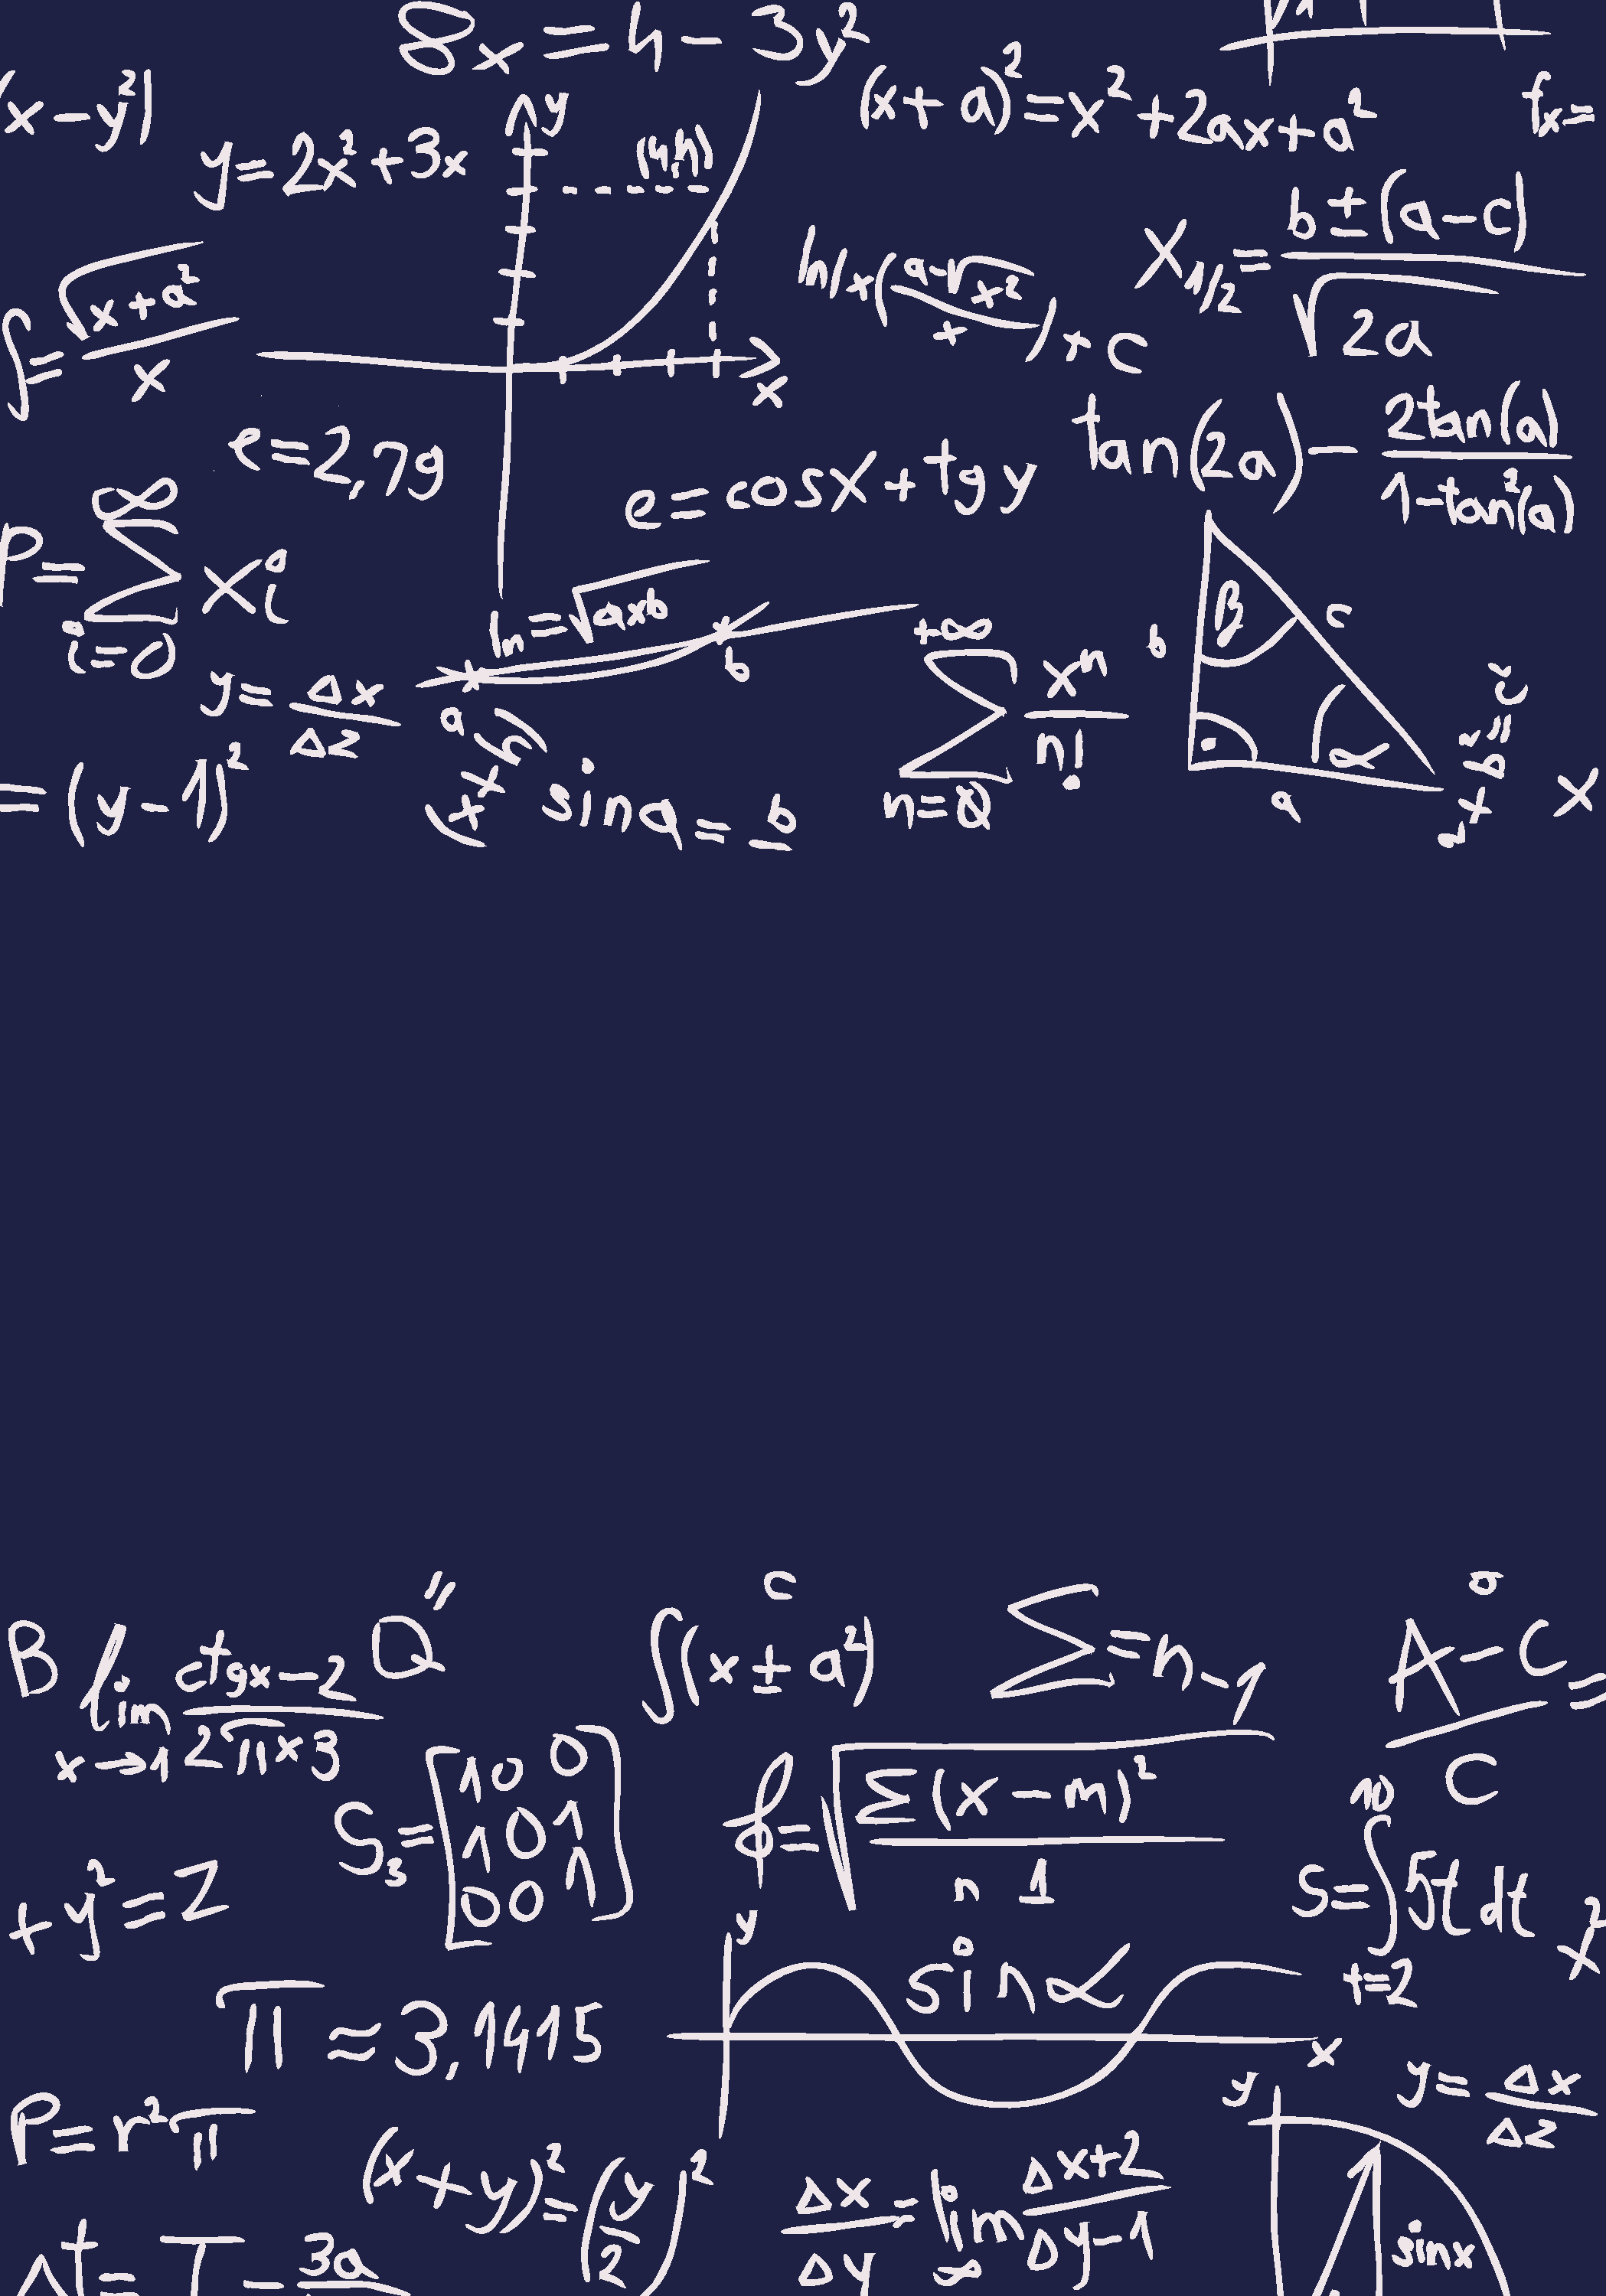
\includegraphics[width=\paperwidth]{Pictures/background.pdf}};
\draw (current page.center) node [fill=blue!30!white,fill opacity=0.6,text opacity=1,inner sep=1cm]{\Huge\centering\bfseries\sffamily\parbox[c][][t]{\paperwidth}{\centering Álgebra Lineal 2\\[15pt] % Book title
{\Large Una aventura en las matemáticas}\\[20pt] % Subtitle
{\huge Rudik Roberto Rompich}}}; % Author name
\end{tikzpicture}
\vfill
\endgroup

%----------------------------------------------------------------------------------------
%	COPYRIGHT PAGE
%----------------------------------------------------------------------------------------

\newpage
~\vfill
\thispagestyle{empty}

\noindent Copyright \copyright\ 2020 Rudik Rompich\\ % Copyright notice

\noindent \textsc{Published by Rudiks}\\ % Publisher

\noindent \textsc{rudiks.com}\\ % URL

\noindent Licensed under the Creative Commons Attribution-NonCommercial 3.0 Unported License (the ``License''). You may not use this file except in compliance with the License. You may obtain a copy of the License at \url{http://creativecommons.org/licenses/by-nc/3.0}. Unless required by applicable law or agreed to in writing, software distributed under the License is distributed on an \textsc{``as is'' basis, without warranties or conditions of any kind}, either express or implied. See the License for the specific language governing permissions and limitations under the License.\\ % License information, replace this with your own license (if any)

\noindent \textit{First printing, October 2020} % Printing/edition date

%----------------------------------------------------------------------------------------
%	TABLE OF CONTENTS
%----------------------------------------------------------------------------------------

%\usechapterimagefalse % If you don't want to include a chapter image, use this to toggle images off - it can be enabled later with \usechapterimagetrue

\chapterimage{Pictures/0002} % Table of contents heading image

\pagestyle{empty} % Disable headers and footers for the following pages

\tableofcontents % Print the table of contents itself

\cleardoublepage % Forces the first chapter to start on an odd page so it's on the right side of the book

\pagestyle{fancy} % Enable headers and footers again

%----------------------------------------------------------------------------------------
%	PART
%----------------------------------------------------------------------------------------

\part{Funcionales lineales}

\chapterimage{Pictures/0001} % Chapter heading image

\chapter{Funcionales lineales}

\section{Ejercicios y Teoremas}

\begin{definition}
Sea $V$ un espacio vectorial sobre $\mathbb{F}$. Entonces, una transformación lineal $$f:V\mapsto\mathbb{F}$$ es un funcional lineal sobre $V$. 
\end{definition}

\begin{exercise}
Sean $\alpha_1,...,\alpha_n \in\mathbb{R}$. Definimos:
$$\Phi:\mathbb{R}^n\mapsto\mathbb{R}\ni$$
$$\Phi(x_1,...,x_n)=\alpha_{1}x_{1}+...+\alpha_{n}x_{n}$$
$\Rightarrow\Phi$ es funcional lineal. 
\end{exercise}
\begin{notation}
$$f:\mathbb{R}^2\mapsto\mathbb{R}\ni$$
$$\Phi(x,y)=2x-y$$
\end{notation}

\begin{exercise}
Sea $C[0,1]$ un conjunto de funciones continuas en [2,1] y considere:
$$T:C[0,1]\mapsto\mathbb{R}\ni$$
$$T(g)=\int^1_0 g(x)dx$$
Nótese si $f,g\in[0,1]$ y $\alpha\in R$$\Rightarrow T(\alpha f+g)=\int^1_0[\alpha f+g](x)dx=\int^1_0[(\alpha f)(x)+g(x)]dx=\alpha\int^1_0f(x)dx+\int^1_0f(x)dx+\int^1_0 g(x)dx=\alpha T[f]+T[g]\Rightarrow$ es lineal $\Rightarrow$ T es funcional lineal. 
\end{exercise}

\begin{exercise}
Sea $$d:\mathbb{R}^{nxn}\mapsto\mathbb{R}\ni$$
$$d(A)=\text{determinante de A}$$
Recordar que: $$det(A+B)\neq det(A)+det(B)$$
$$det(\alpha A)\neq \alpha det(A)$$
$$d(A) \text{ no es funcional lineal}$$
\end{exercise}

\begin{exercise}
Sea $$T:\mathbb{R}^{nxn}\mapsto\mathbb{R}\ni$$
$$T(A)=\text{ traza de A}$$
$$\text{Si } A=[a_{ij}]\Rightarrow Tr(A) = \sum^n_{i=1}a_{ij}$$
$$\Rightarrow Tr(A) \text{ es funcional lineal.}$$
\end{exercise}
\begin{exercise}
Sea $V$ el espacio de todas las funciones sobre $\mathbb{R}$.
Definimos $$C_t: V\mapsto\mathbb{R}\ni$$
$$C_t(f)=f(t)\text{ , donde t es un número fijo.}$$
Nótese que:
\begin{enumerate}
    \item Sea $f,g\in V\Rightarrow L_t[f+g]=(f+g)(t)=L_t(f)+L_t(g)$
    \item Sea $\alpha\in\mathbb{R}\mapsto L_t(\alpha f)=(\alpha f)(t)=\alpha f(t)=\alpha L_t(f)\Rightarrow\text{ Es funcional lineal.}$
\end{enumerate}
\end{exercise}

\begin{notation}
Considere el funcional lineal $$f:\mathbb{R}^n\mapsto\mathbb{R}\ni$$$$f(x_1,...,x_n)=\alpha_1 x_1+...+\alpha_n x_n.$$
$$ \alpha_1\in\mathbb{R}$$ (fijos)
Sea $B=\{e_1,...,e_n\}$ la base usual de $\mathbb{R}^n$ y sea $B'=\{1\}$ la base usual de $\mathbb{R}$. $$f(1,0,...,0)=\alpha_1(1)+\alpha_2(0)+...+\alpha_1(0)$$
$$=\alpha_1$$
$$f(0,1,0,...,0)=\alpha_2$$
$$\vdots$$
$$\Rightarrow[f]^{B'}_B =[\alpha_1\,\alpha_2\,...\,\alpha_n]$$

\end{notation}

\begin{notation}
Si $f$ son funcionales lineales. 
$$f\in f[V,\mathbb{F}]\text{ si dim(V)=n}$$
$$\Rightarrow dim( f[V,\mathbb{F}])= n\cdot1=n$$
\end{notation}

\begin{definition}[$V^{*}$]
Al espacio de funciones lineales de V es $\mathbb{V}$ es $\mathbb{F}$ se le llama al espacio dual de $V$.
\end{definition}

\begin{notation}
Si $dim(V)=n \Rightarrow dim(V^*)=n$
\end{notation}

\subsection{Teorema}
\begin{theorem}
Sea $V$ un espacio vectorial finito dimensional y $B=\langle v_1,...,v_n\rangle$ una base ordenada de $V$. Entonces, existe una base: $B^* = \{\Phi_1,...,\Phi_n\}$ de $V^*$, tal que: 
$$\Phi_i(V_j)=
    \begin{cases} 
      1 & i=j \\
      0 & i\neq j  
   \end{cases} = \delta_{ij} $$
$$\Phi_i(V_j)=\delta_{ij}\xleftarrow{\text{ Delta de Kronecker}}$$


\end{theorem}

\subsection{Ejercicio}
\begin{exercise}
Considere la base de $\mathbb{R}^2$,
$$B=\{(2,1),(3,1)\}$$
entonces, encuentre una base para para $(\mathbb{R^2})^{*}\xleftarrow{\mathcal{L}[\mathbb{R}^2,\mathbb{R}^2]}$
\end{exercise}

\textbf{Solución:}
\begin{align}
    B^* &= \{\phi_1,\phi_2\} & \text{es tal que:}\\
    \intertext{Debemos encontrar $\alpha_1,\alpha_2,\beta_1,\beta_2$}
    \phi_1(x,y)&=\alpha_1 x+\alpha_2 y\\ 
    \phi_2(x,y)&=\beta_1 x+\beta_2 y\\
    \intertext{Encontramos $\alpha_1 y \alpha_2$:}
    \phi_1(v_1)&=\phi(2,1)=2\alpha_1+\alpha_1=1  & \delta_{11}\\
    \phi_1(v_2)&=\phi(3,1)=3\alpha_1+\alpha_2=0  & \delta_{11}\\
    \implies &\alpha_1=-1, \alpha=3\\
    \implies & \phi_1(x,y)=-x+3y\\
    \intertext{Encontramos $B_1,B_2$:}
    \phi_2(v_1)=\phi_2(2,1)= 2\beta_1+\beta_2 =0\\ 
    \phi_2(v_2)=\phi_2(3,1)= 3\beta_1+\beta_2 =1\\
    \implies & \beta_1=1,\beta_2=-2\\
    \implies &\phi_2(x,y) =x -2y 
\end{align}
$\implies$ La base dual de $B$, denotada por $B^*$ (i.e. la base del espacio dual $V^)*$, es \\$B^{*}=\{-x+3y,-x+2y\}$

\subsection{Ejercicio}
\begin{exercise}
Dada la base de $\mathbb{R}^3$:\\
$$B=\{(1,-1,3),(0,1,-1),(0,3,-2)\},$$
encuentre la base dual de $B^*$ (i.e. la basa para $\mathcal{L}[\mathbb{R}^3,\mathbb{R}]$)
\end{exercise}


\begin{align}
    \phi_1(x,y,z)&=\alpha_1 x +\alpha_2 y+\alpha_3 z\\
    \phi_2(x,y,z)&=\beta_1 x +\beta_2 y+\beta_3 z\\
    \phi_3(x,y,z)&=\gamma_1 x +\gamma_2 y+\gamma_3 z\\
    \intertext{Encontramos $\alpha_1,\alpha_2,\alpha_3$: }
    \p_1(v_1)&=\p_1(1,-1.3)=\al_1-\al_2+2\al_3=1\\
    \p_2(v_2)&=\p_1(0,1,-1)=0\al_1+\al_2 -1\al_3=0\\
    \p_3(v_3)&= \p_1(0,3,-2)=0\al_1+3\al_2-2\al_3=0\\
    \implies &\al_1=1,\al_2=\al_3=0 \implies \p_1(x,y,z)=x
    \intertext{Encontramos $\be_1,\be_2,\be_3$:}
    \p_2(v_1)&=\p_2(1,-1,3)=1\be-1\be+2\be= 0\\
    \p_2(v_2)&=\p_2(0,1,-1)=0\be+1\be-1\be= 1\\
    \p_2(v_3)&=\p_2(0,3,-2)=0\be+3\be-2\be= 0\\
    \implies &\be_1=7,\be_2=-2,\be_3=-3 \implies \p_2(x,y,z)=7x-2y-3z
    \intertext{Encontramos $\g_1,\g_2,\g_3$}
    \p_3(v_1)&=\p_3(1,-1,3)=1\g-1\g+2\g= 0\\
    \p_3(v_2)&=\p_3(0,1,-1)=0\g+1\g-1\g= 1\\
    \p_3(v_3)&=\p_3(0,3,-2)=0\g+3\g-2\g= 0\\
    \implies &\g_1=2,\g_2\g_3=1 \implies \p_3(x,y,z)=-2x+y+z
    \intertext{Por lo tanto:}
    B^* &= \{x,7x-2y-3z,-2x+y+z\}
    \intertext{Por otra parte, es necesario probar que $B^*$ es linealmente independiente}
    \text{Considere: }& \up_1\p_1+\up_2\p_2+...+\up_n\p_n =0\\
    \text{A probar: }& \up_1=\up_2=...=\up_n=0\\
    \intertext{Sea $v_i\in B$, $1\leq i\leq n$}
    \implies & (\up_1\p_1+...+\up_1\p_i+...+\up_n\p_n)(v_i)=0(v_i)\\
    \implies & \up_1\p_1(v_i)+...+\up_1\p_i(v_i)+...+\up_n\p_n)(v_i)=0\\
    \implies & 0+1 +0 &= 0\\
    \implies &\up_1=\up_2=...=\up_n=0 \implies \{\p_1,...,\p_n\}\text{ es linealmente independiente}\\
\end{align}

\subsection{Teorema}
\begin{theorem}
Sea $V$ un espacio vectorial finito dimensiona y sea $B=\{x_1,...,x_2\}$ una base ordenada para $V$. Entonces existe una base $B^* = \{\p_1,...,\p_n \}$ para $V^* \ni$ $$\p_i(x_j)=\delta_ij$$
Además, 
\begin{align}
    \intertext{(i) $\forall \p \in V^*$ se tiene:}\\
    \p =\p(x_1)\p_1+\p(x_2)\p_2+...+\p(x_n)\p_n\\
    \intertext{(ii) $\forall x \in V$ se tiene que:}\\
    x=\p_1(x)x_1+\p_2(x)x_2+...+\p_n(x)x_n\\
\end{align}
\end{theorem}

\begin{proof}
\begin{align}
    \intertext{A probar: $B^*$ es linealmente independiente. Considere:}\\
    \al_1\p_1+...+\al_n\p_n &=0_n \\
    \text{funcional lineal} &= \text{funcional lineal}\\
    \intertext{Aplicando a $x_i (i=1,...,n)$}\\
    (\al_1\p_1+...+\al_i\p_i+...+\al_n\p_n)(x_j)\\
    \implies \alpha_1\p_1(x_i)+...+\alpha_i\p_i(x_i)+...+\al_n\p_n(x_i)=0\\
    \implies \alpha_i =0  \\
    \implies B^* \text{ es linealmente independiente.}
    \intertext{(2)$B^*$ genera a $V^*$}
    \intertext{Sea $\phi\in v^*$. Entonces, sean:}
    \p(x_1)=\la_1,\p(x_2)=\la_2,...,\p(x_n)=\la_n\\
    \intertext{Por otro lado, hagamos:}
   \sigma = \la_1\p_1+\la_2\p_2+...+\la_n\p_n\\
   \implies \sigma(x_1) &= (\la_i\p_1+...+\la_n\p_n)(x_1)\\
    &= \la_1\p_1(x_1)+\la_2\p_2(x_1)+...+\lambda_n\p_n (x_1)\\ 
   &= \la_1 + 0+0\\
    \intertext{De la misma forma: }
    \sigma(x_i)=\la_i\\
    \implies \p(x_i)=\sigma(x_i) \\
   \implies \p = \sigma=\la_1\p_1+\la_2\p_2+...+\la_n\p_n\\
   \intertext{(ii) Sea $x\in V\implies x=\al_1 x_1+...+\al_n x_n$, donde $\al_1,...,\al_n \in \mathbb{F}$}
   \implies \p_1(x)&= \p_1(\al_1 x_1+...+\al_n x_n)\\
   &= \al_1\p_1(x_1)+\al_2\p_1(x_2)+...+\al_n\p_1(x_n)\\
   \implies \p_1(x)&=\al_1\\
   \intertext{En general, $\p_i(x)=\al_i, i=1,...,n$}
   \implies x=\al_1 x_1 +\al_2 x_2 +...+\al_n x_n\\
   \implies x=\p_1(x)x_1 +\p_2(x)x_2+\p_n(x)x_n\\
   \intertext{Sea $x\in V \implies x=\p_1(x)x_1+...+\p_n(x)x_n$}
   \intertext{Si $\p\in V^*$, entonces: }
   \p_(x) &= \p[\p_1 (x)x_1 +...+\p_n (x)x_n]\\
   &= \p_1 (x)*\p(x_1)+...+\p_1 (x) \p(x_1)\\
   &= \p(x_1)\p_1(x)+...+\p(x_2)\p(x)\\
   &= [\p(x_1)\p_1 +\p(x_2)\p_2+...+\p(x_n)\p_n](x)\\
   \implies \p=\p(x_1)\p_1+...+\p(x_2)\p_n
\end{align}
\end{proof}
\newpage

\subsection{Ejercicio}

\begin{exercise}
\begin{align}
    \intertext{Sea:}
    \mathbb{R}_1 [x]=\s{a+bx: a,b\in\mathbb{R}}\\
    \intertext{Sean:}
    \p_1: V\mapsto \mathbb{R} \text{  y  }\p_2:V\mapsto\mathbb{R}\ni\\
    \p_1(f(x))=\ie{0}{1}{f(x)}{x} \text{  ,  } \p_2(f(x))= \ie{0}{2}{f(x)}{x}\\
    \text{Encuentre una base }B=\s{f1,f2} \text{ cuya base dual es: } B^* = \s{\p_1,\p_2} 
\end{align}
\end{exercise}

\begin{proof}
\begin{align}
    \intertext{Sean:}
    f_1= a+bx\\
    f_2= c+dx\\
    \p_1(f_1)&=1=\ie{0}{1}{a+bx}{x}=ax+\frac{1}{2}bx^2 |_0^1 =1\\
    \p_2(f_1)&=0=\ie{0}{2}{a+bx}{x}=ax+\frac{1}{2}bx^2 |_0^2 =0\\
\end{align}
\begin{align}
    a+\frac{1}{2}b=1\\
    2a+2b=0\\
    \implies a=2,b=-2\\
    \implies f_1 = 2-2x\\
\end{align}

\begin{align}
\p_1(f_1)=0=\ie{0}{1}{c+dx}{x}=c+\frac{1}{2}d\\
\p_2(f_2)=1=\ie{0}{2}{c+dx}{x}=2c+2d\\
\implies& c+\frac{1}{2}d = 0\\
&2c+2d=1\\
\implies c=\frac{-1}{2}, d=1\\
\implies f_2 = \frac{-1}{2} +x\\
\therefore B=\s{1-1x,\frac{-1}{2}+x}
\end{align}
\end{proof}

\subsection{Ejercicio (***)}

\begin{exercise}
\begin{align}
    \intertext{Sea}
    && V= \mathbb{R}_2 [x]=\s{a+bx+cx^2, a,b,c\in\mathbb{R}^2}&&\\
    \intertext{Nótese que $dim(\mathbb{R}_2 [x])=3$}\\
    \text{Una base para $\mathbb{R}$ es $1,x,x^2$}\\
\end{align}
\end{exercise}
\begin{remark}
No se prueba que genera ya que dim=3
\end{remark}
\begin{proposition}
\begin{align}
     \intertext{(i) Considere $\al_1,\al_2,\al_3$ números reales diferentes y definimos:}\\
    &&L_i : \mathbb{R}_2[x]\mapsto\mathbb{R}\ni && i=1,2,3\\
    &&L_i (p) := p(\al_i)&&\\
    \intertext{Los $L_i$ son funcionales lineales. En efecto, sean $p,q \in \mathbb{R}_2 [x]$ y $\al \in \mathbb{R}$. Entonces:}
    && L_i(\al p+1) &= (\al p +1)(\al_i) = \al p(x_i)+q(\al_i)&&\\
    && &= \al L_i(p)+L_i(q)&&\\
    \implies L_i \text{ es funcional lineal}, i=1,2,3\\
\end{align}

\begin{align}
    \intertext{(ii) $\s{L_1,L_2,L_3}$ es linealmente independiente}
    &&V &= \mathbb{R}_2[x]&\implies B=\s{\space,\space,\space}&&\\
    &&V^* &= &\implies B^* =\s{L_1,L_2,L_3}&&\\
    \intertext{Considere: }
    \mi{\be_1 L_1 + \be_2 L_2+\be_3 L_3 =0}\\
    Si p_1(x) = 1 \implies \mi{(\be_1L_1+\be_2 L_2 +\be_3 L_3) (p_1)=0 (p_1)}\\
    \implies \mi{\be_1 L_1(p_1)+\be_2 L_2(p_1) +\be_3 L_3 (p_1)=0}\\
    \implies \mi{\be_1 p_1 (\al_1)+\be_2 p_1(\al_2)+\be_3 p_1(\al_3)=0}\\
    \implies \mi{\be_1(1)+\be_2(1)+\be_3(1)=0}\\
    \implies \mi{\be_1+\be_2+\be_3 =0}
    \intertext{$\s{L_1,L_2,L_3}$ es linealmente independiente $\implies \s{L_1,L_2,L_3}$ es una base para $V^*$}
    \end{align}
    \begin{align}
        \intertext{(iii) Encuentra la base para $V$ de la $\s{L_1,L_2,L_3}$ es dual}
        \text{Si } p_1(x)=1,p_2(x)=x\\
        \implies \mi{(\be_1 L_1 + \be_2 L_2 +\be_3 L_3)(p_2)=0(p_2)}\\
        \implies \mi{\be_1 L_1(p_2) + \be_2 L_2 (p_2) +\be_3 L_3(p_2)=0}\\
        \implies \mi{\be_1\al_1 +\be_2\al_2+\be_3\al_3 =0}\\
        \intertext{Si $ p_1(x)=1,p_2(x)=x,p_3(x)=x^3$}
        \implies \mi{(\be_1 L_1+\be_2 L_2 +\be_3 L_3)p_3 =0p_3}\\
        \implies \mi{\be_1 L_1 (p_3)+ \be_2 L_2 (p_3) +\be_3 L_3 (P_3) =0}\\
        \implies \mi{\be_1 \al_1^2 +\be_2\al_2 ^2 + \be_3 \al_3^2 =0}
    \end{align}
    \begin{align}
        \intertext{Se tiene el sistema:}
        \mi{\be_1+\be_2+\be_3 =0}\\
        \mi{\al_1\be_1+\al_2\be_2+\al_3\be_3 =0}\\
        \mi{\al_1^2\be_1+\al_2^2\be_2+\al_3^2\be_3=0}\\
        \intertext{Es decir, matricialmente:}
        \mi{\begin{pmatrix}
        1 & 1 &1\\ \al_1 &\al_2&\al_3\\ \al_2^2 & \al_2^2 &\al_3^2 
        \end{pmatrix}\begin{pmatrix}\be_1\\\be_2\\\be_3\end{pmatrix}=\begin{pmatrix}0\\0\\0
        \end{pmatrix}}\\
        \intertext{Si $\al_1,\al_2,\al_3$ son distintos, entonces:}
        \mi{det\begin{pmatrix}
        1 & 1 &1\\ \al_1 &\al_2&\al_3\\ \al_2^2 & \al_2^2 &\al_3^2 
        \end{pmatrix}\neq 0 \implies \begin{pmatrix}\be_1\\\be_2\\\be_3\end{pmatrix}=\begin{pmatrix}0\\0\\0
        \end{pmatrix}}\\
        \implies \mi{(\al_1-\al_2)(\al_2-\al_3)(\al_3-\al_1)=0}\\
        \implies \mi{\s{L_1,L_2,L_3}\text{ es linealmente independiente}}\\
        \implies \s{L_1,L_2,L_3} \text{ es una base para $V^*$}
    \end{align}
\end{proposition}

\subsection{Ejercicio}
\begin{exercise}
\begin{align}
    \intertext{$\s{f_1,f_2,f_3}$ de $\mathbb{R}_2[x]$, tal que una base dual $B^*=\s{L_1,L_2,L_3}$}
    \intertext{Nótese que:}
    \mi{L_i(f_j)=\delta_{ij}}\\
    \p_i(x_j) =\delta{ij}\implies \mi{f_j(\al_i)=\delta_{ij}}\\
    \mi{f_1(\al_{2j})=\delta_{ij}}\\
    \mi{f_2(\al_i)=\delta_{ij}}
    \intertext{Esto quiere decir:}
    \mi{f_1(x) &= \frac{(x-\al_2)(x-\al_3)}{(\al_1-\al_2)(\al_1-\al_3)}}\\
    \implies \mi{f_1(\al_1)=1,f_2(\al_2)=f_3(x_3)=0}\\
    \implies \mi{f_1(\al_i)=\delta_{ij}}\\
    \mi{f_2(x)=\frac{(x-\al_1)(x-\al_3)}{(\al_2-\al_1)(\al_2-\al_3)}}\\
    \mi{f_3(x)= \frac{(x-\al_1)(x-\al_2)}{(\al_3-\al_1)(\al_3-\al_2)}}\\
    \text{Polinomios de Lagrange}
\end{align}
\end{exercise}

\subsection{Ejercicio}
\begin{exercise}
\begin{align}
\intertext{Dados:}
\mi{L_i = \mathbb{R}_2[x]\mapsto \mathbb{R}\ni}\\
\mi{L_i(p)= p(\al_i)}\\
\intertext{$L_i$ son funcionales lineales.}\\
\intertext{$\s{L_1,L_2,L_3}$ es linealmente independiente $\implies$ es base de $(\mathbb{R}_2 [x])^*$}\\
\intertext{Se debe cumplir: }
\mi{L_i(p_j)=\delta_{ij}}\\
<=> \mi{p_j(\al_i)=\delta_{ij}}\\
\implies \mi{p_j(\al_i)= \begin{cases}1 & \text{si $j= i$} \\0 & \text{si $j\neq i$}\end{cases}}
\end{align}
\end{exercise}

\begin{proof}
\begin{align}
\intertext{¿Quiénes son $\al_1,\al_2,\al_3$?}
    \mi{p_1(\al_1)=1 & p_1(\al_2)=0 & p_1(\al_3)=0 }\\
    \mi{p_2(\al_1)=0 & p_2(\al_2)=1 & p_2(\al_3)=0 }\\
    \mi{p_3(\al_1)=0 & p_3(\al_2)=0 & p_3(\al_3)=1 }\\
    \implies \mi{p_1(x) = \frac{(x-\al_2)(x-\al_3)}{(\al_1-\al_2)(\al_1-\al_3)}}\\
    \mi{p_2(x)=\frac{(x-\al_1)(x-\al_3)}{(\al_2-\al_1)(\al_2-\al_3)}}\\
    \mi{p_3(x)= \frac{(x-\al_1)(x-\al_2)}{(\al_3-\al_1)(\al_3-\al_2)}}
    \intertext{$\s{p_1(x),p_2(x),p_3(x)}$ es la base de $R_2 [x] \ni \s{L_1,L_2,L_3}$ es una base dual. Además, si $p\in \mathbb{R}_2 [x]$; entonces, $p=p(\al_1)p_1+p(\al_2)p_2 +p(\al_3)p_3$ (Polinomio interpolante de Lagrange).}
\end{align}
\end{proof}


\tikzset{every picture/.style={line width=0.75pt}} %set default line width to 0.75pt        

\begin{tikzpicture}[x=0.75pt,y=0.75pt,yscale=-1,xscale=1]
%uncomment if require: \path (0,300); %set diagram left start at 0, and has height of 300

%Shape: Axis 2D [id:dp4548434535748712] 
\draw  (156,247.67) -- (479.64,247.67)(188.36,10) -- (188.36,274.08) (472.64,242.67) -- (479.64,247.67) -- (472.64,252.67) (183.36,17) -- (188.36,10) -- (193.36,17)  ;
%Curve Lines [id:da9088123433049421] 
\draw    (246.93,176.87) .. controls (307.55,42.4) and (395.55,87.77) .. (419.02,180.11) ;
%Flowchart: Connector [id:dp8788809565179998] 
\draw  [fill={rgb, 255:red, 255; green, 0; blue, 0 }  ,fill opacity=1 ] (321.24,91.01) .. controls (321.24,84.74) and (327.15,79.67) .. (334.44,79.67) .. controls (341.73,79.67) and (347.64,84.74) .. (347.64,91.01) .. controls (347.64,97.27) and (341.73,102.35) .. (334.44,102.35) .. controls (327.15,102.35) and (321.24,97.27) .. (321.24,91.01) -- cycle ;
%Flowchart: Connector [id:dp8954838959032968] 
\draw  [fill={rgb, 255:red, 255; green, 0; blue, 0 }  ,fill opacity=1 ] (233.73,176.87) .. controls (233.73,170.61) and (239.64,165.53) .. (246.93,165.53) .. controls (254.22,165.53) and (260.13,170.61) .. (260.13,176.87) .. controls (260.13,183.14) and (254.22,188.22) .. (246.93,188.22) .. controls (239.64,188.22) and (233.73,183.14) .. (233.73,176.87) -- cycle ;
%Flowchart: Connector [id:dp6810968886330147] 
\draw  [fill={rgb, 255:red, 255; green, 0; blue, 0 }  ,fill opacity=1 ] (405.82,180.11) .. controls (405.82,173.85) and (411.73,168.77) .. (419.02,168.77) .. controls (426.31,168.77) and (432.22,173.85) .. (432.22,180.11) .. controls (432.22,186.38) and (426.31,191.46) .. (419.02,191.46) .. controls (411.73,191.46) and (405.82,186.38) .. (405.82,180.11) -- cycle ;
%Straight Lines [id:da6329359783579342] 
\draw    (167.73,180.11) -- (207.82,180.11) ;
%Straight Lines [id:da14731564882391568] 
\draw    (245.95,267.6) -- (246.93,235.2) ;
%Straight Lines [id:da2945881029344082] 
\draw    (337.86,267.6) -- (338.84,235.2) ;
%Straight Lines [id:da4835859670975893] 
\draw    (421.95,267.6) -- (422.93,235.2) ;

% Text Node
\draw (282.19,148.43) node [anchor=north west][inner sep=0.75pt]    {$p( \alpha _{1})$};
% Text Node
\draw (299.79,46.36) node [anchor=north west][inner sep=0.75pt]    {$p( \alpha _{2})$};
% Text Node
\draw (466.01,158.15) node [anchor=north west][inner sep=0.75pt]    {$p( \alpha _{3})$};
% Text Node
\draw (239.87,268.32) node [anchor=north west][inner sep=0.75pt]    {$\alpha _{1}$};
% Text Node
\draw (333.73,266.7) node [anchor=north west][inner sep=0.75pt]    {$\alpha _{2}$};
% Text Node
\draw (415.86,265.08) node [anchor=north west][inner sep=0.75pt]    {$\alpha _{3}$};


\end{tikzpicture}
\part{Aniquiladores}

\chapterimage{Pictures/0001} % Chapter heading image

\chapter{Aniquiladores}


\end{document}